 %2
\section{\system}
\label{repiano}

{\system}は、自分の過去の演奏履歴を活用することによって演奏をより楽しくすることができるシステムである。
演奏中に以下のボタンを押すことで楽しい演奏ライフをサポートする。

%2.1
\subsection{録音再生ボタン}
\label{recplaybutton}

直前の無音部分から現在までの演奏を登録して、繰り返し再生を行う。(\figref{recplay1})
録音開始の操作は不要で、演奏の途中や、
演奏が終わってから登録可能な点が既存のツールとは異なる大きな特徴である。
登録部分の中に演奏の繰り返しが含まれる場合はDynamic Macro\cite{masui}を適用し、
繰り返し部分だけを登録して連続再生を行う。(\figref{recplay2})
また、再生中に重ねて演奏を行なうことができ、そこで録音再生ボタンを押すとその演奏も新たに登録される。
この演奏は最初に登録された繰り返しフレーズのタイミングに合わせて記録されるため、
時間が経過してもずれることなく再生され続ける。

\begin{figure}[tb]
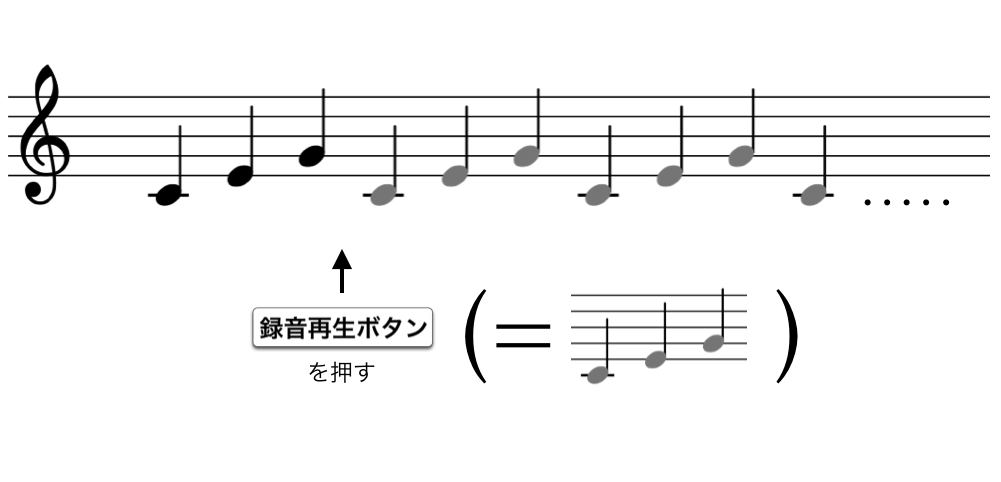
\includegraphics[width=8cm,bb=0 0 1054 481]{images/rp1.png}
\centering
\caption{演奏の登録}
\label{recplay1}
\end{figure}

\begin{figure}[tb]
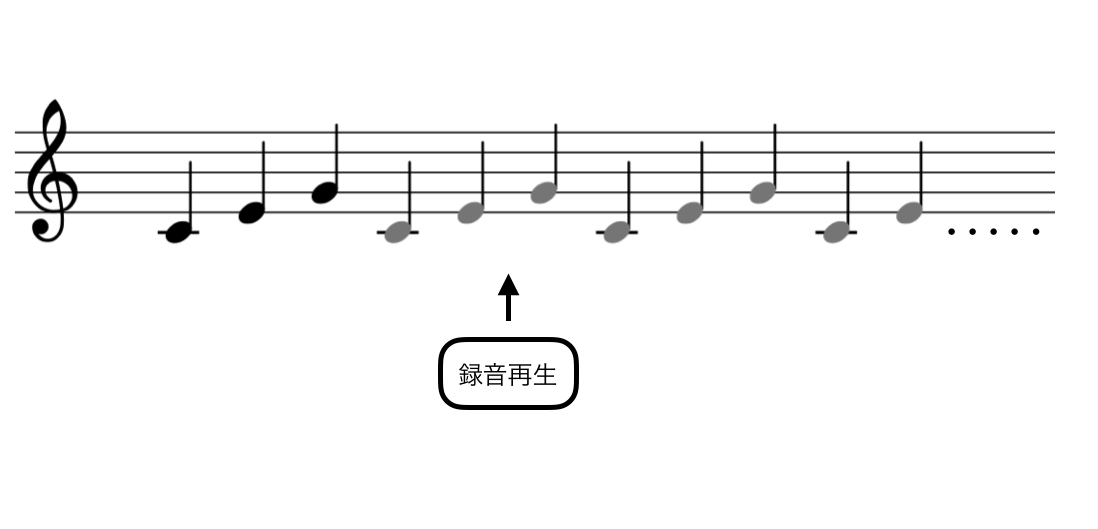
\includegraphics[width=8cm,bb=0 0 1054 481]{images/rp2.png}
\centering
\caption{Dynamic Macroの適用}
\label{recplay2}
\end{figure}

%2.2
\subsection{やり直しボタン}

\ref{recplaybutton}で重ねていった演奏を、新しいものから順に取り消す。
登録された演奏はそれぞれ独立して管理されているので、
やり直しボタンによってすぐ以前の状態に戻すことができる。
